\section{设计与框架}

\subsection{源代码组织}

总体来说,所有源代码都在\verb|src|文件夹下,为:
\begin{lstlisting}
./src
|-- argparse
|   `-- argparse.go
|-- list
|   `-- list.go
|-- logic
|   `-- logic.go
|-- main.go
|-- parse
|   |-- parse.go
|   `-- parse.y
`-- units
    |-- file.go
    |-- split.go
    |-- version.go
    `-- wordmap.go

5 directories, 10 files
\end{lstlisting}

按照模块化结构,所有的源代码都分工合作,各司其职。分别对他们进行
短暂描述:

\textline

\begin{description}[labelindent=\parindent]
    \item[argparse:] 解析命令行命令,提供usage提示。
    \item[list:] 提供有序链表的接口。
    \item[logic] 实现了底层,如根据抽象出的语法树处理业务
        进行搜索处理。
    \item[parse:] 将前端的命令处理为抽象语法树。
    \item[units:] 杂项。
        \begin{description}
            \item[file:] 提供处理文件的接口。
            \item[spilt:] 提供文本分词的接口,用来将文件转
                换为数据结构,它是是处理index文件的第一步。
            \item[version:] 提供版本信息。
            \item[wordmap:] 抽象出的最主要的数据结构。储存了
                单词的在文件中出现过的位置。
        \end{description}
\end{description}

\textline

\subsection{整体逻辑组织}

整体上来说逻辑分层,分别分为I/O层,Mid层\footnote{用来处理大部分
逻辑,包括,处理从I/O中传入的数据,使用Low层作为工具进行逻辑处理,
返回Low层数据结构},Low层\footnote{定义和抽象绝大多数的数据结构。}%
和Sys层\footnote{如内存管理等等。使用\go 语言操控,并没有实际接触。}。
大体来说,整体的逻辑组织结构如图\ref{struct}。

\begin{figure}[H]
\centering
\tikzstyle{outer} = [rectangle, draw=black!50, fill=black!20, thick,
                     minimum size=6mm, minimum width=10em, rounded corners]
\tikzstyle{inter} = [rectangle, draw=blue!50, fill=blue!20, thick,
                     minimum size=6mm, minimum width=10em, rounded corners]
\tikzstyle{labal} = [auto, swap, align = left]
\tikzstyle{biglabel} = [align = right, left]
\tikzstyle{bigline} = [very thick, black!50]
\setlength{\fboxsep}{1em}
\footnotesize
\fbox{%
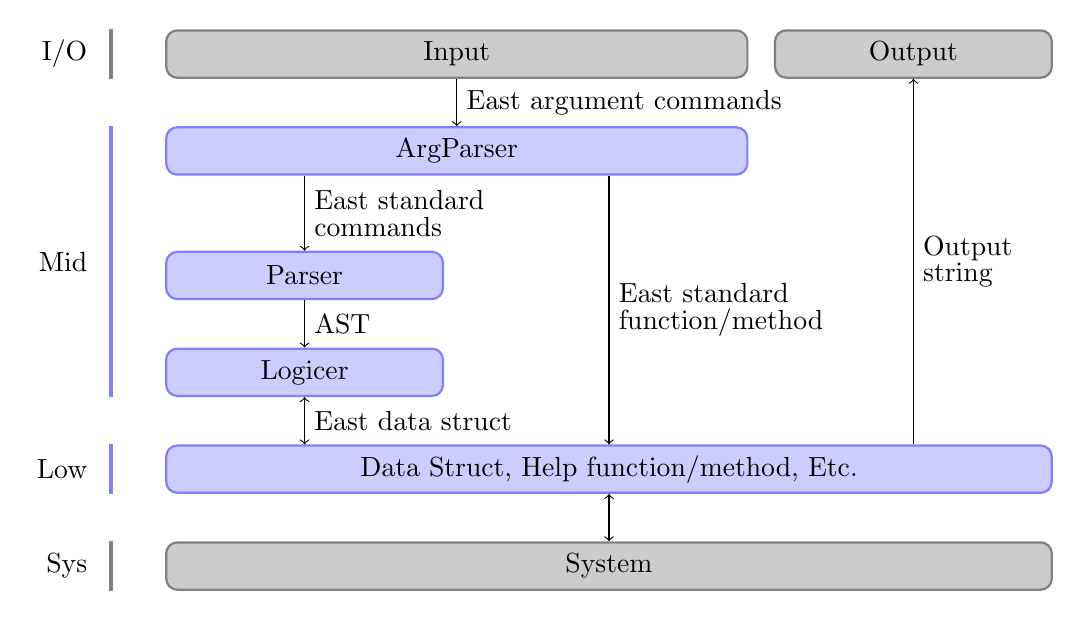
\begin{tikzpicture}
    \setlength{\baselineskip}{0.8\baselineskip}
    \node (command)   at (5.5em, 0)          [outer, minimum width = 21em] {Input};
    \node (screen)    at (22em, 0)           [outer] {Output};
    \node (argparse)  at (5.5em, -3.5em)     [inter, minimum width = 21em] {ArgParser}
          edge [<-] node[labal] {East argument commands} (command);
    \node (parser)    at (0, -8em)           [inter] {Parser}
          edge [<-] node[labal] {East standard\\commands} (argparse.south -| parser);
    \node (logicer)   at (0, -11.5em)        [inter] {Logicer}
          edge [<-] node[labal] {AST} (parser);
    \node (low level) at (11em, -15em)       [inter, minimum width = 32em]
                                             {Data Struct, Help function/method, Etc.}
          edge [<-] node[labal] {East standard\\function/method}
                                             (argparse.south -| low level)
          (low level.north -| logicer) edge [<->] node[labal] {East data struct} (logicer)
          (low level.north -| screen) edge [->] node[labal] {Output\\string} (screen);
    \node (system)    at (11em, -18.5em)     [outer, minimum width = 32em] {System}
          edge [<->] node[labal] {\go} (low level);

    \node (IO)  at (-7.5em, 0)       [biglabel] {I/O};
    \node (Mid) at (-7.5em, -7.5em)  [biglabel] {Mid};
    \node (Low) at (-7.5em, -15em)   [biglabel] {Low};
    \node (Sys) at (-7.5em, -18.5em) [biglabel] {Sys};

    \draw [bigline] (command.north -| -7em, 0)   -- (command.south -| -7em, 0);
    \draw [bigline, blue!50] (argparse.north -| -7em, 0)  -- (logicer.south -| -7em, 0);
    \draw [bigline, blue!50] (low level.north -| -7em, 0) -- (low level.south -| -7em, 0);
    \draw [bigline] (system.north -| -7em, 0)    -- (system.south -| -7em, 0);
\end{tikzpicture}
}
\caption{the struct of East}
\label{struct}
\end{figure}

\subsection{逻辑结构细节}

为了处理好tf-idf的逻辑细节,我认为,需要一下几点:讲一个文件处理
为一个数组,然后再通过数组构建出初步的词典。将它,和运算后的df处
理好之后,就是一个成熟的解决方案了。

